\documentclass[preprint,12pt,eqsecnum,nofootinbib,amsmath,amssymb]{revtex4}

% Date file was last changed:
\newcommand{\datechange}{Aug 21 2019}
\newcommand{\datestart}{21 Aug 2019}

% version
\newcommand\draftverson{v1.0}
\newcommand{\fname}{spectrum\_preserving\_embedding.tex}
\newcommand{\draftv}{\draftverson}
%\newcommand{\laurnumber}{LA-UR-18-xxxx: \draftverson: \today ~\currenttime}
\newcommand{\laurnumber}{LA-UR-xx-xxxx}
\newcommand{\mydate}{ \datechange}

% v4.3 3/11/2018
% Almost complete version. Needs a new Abstract and better intro to Sec I
% Needs conclusions. Do we want to include energy contours?
% v4.4 3/11/2018
% Move abstract to the intro and shorten.
% v4.4 Theory section
% v4.5 Merge results section
% v4.6 Merge with final results
% v4.7 Merge with latest final results
% v4.8 Final version.
%
% Person who last changed file:
\newcommand{\whochange}{Michael Rogers}
%
% Project Name, path, informal author names, title
\newcommand{\projname}{Quantum Computing}
\newcommand{\dirname}{mygit\_repos/embedding_notes}
\newcommand{\myauthors}{Michael L. Rogers}
\newcommand{\myrunningtitle}{\fname}
\newcommand{\mytitle}{Spectrum Preserving QUBO Embeddings on a Quantum Annealer}
%
% printing margins
%
\textwidth=6.5in
\textheight=9in
%
% packages
%
\usepackage{graphicx}  % Include figure files
\usepackage{dcolumn}  % Align table columns on decimal point
\usepackage{bm}          % Bold math: $\bm{\alpha}$
\usepackage{latexsym}  % Several additional symbols
\usepackage{fancyhdr}  % Fancy header package
\usepackage{wrapfig}
\usepackage{comment}
\usepackage{dsfont}
\usepackage{mathtools}
\usepackage{datetime}
%\usepackage{showkeys}% Displays equation and fig names
%\usepackage{hyperref}% Hyperlinked references

% local commands
\newcommand{\overoverline}[1]{ {\overline{\overline{#1}}} }
\newcommand{\EMPTYSET}{\varnothing}
\newcommand{\PROOF}{{\tiny PROOF}}
\newcommand{\PAR}{$\blacktriangleright$}
\newcommand{\ENDPF}{\blacksquare}
\newcommand{\AND}{\wedge}
\newcommand{\OR}{\vee}
\newcommand{\NOT}{\neg}
\newcommand{\IFF}{\leftrightarrow}
\newcommand{\IMP}{\rightarrow}
\newcommand{\T}{{\rm T}}
\newcommand{\F}{{\rm F}}
\newcommand{\smDash}{{\rule[1mm]{0.1cm}{0.1mm}}}
\newcommand{\dbar}{{d\hskip-0.12cm \rule[2.2mm]{0.15cm}{0.1mm}}}
\newcommand{\calA}{{\cal A}}
\newcommand{\smA}{{\scriptscriptstyle \rm A}}
\newcommand{\smB}{{\rm\scriptscriptstyle B}}
\newcommand{\smN}{{\rm\scriptscriptstyle N}}
\newcommand{\bvec}[1]{\mathbf{#1}}
\newcommand{\smP}{{\rm\scriptscriptstyle P}}
\newcommand{\smL}{{\rm\scriptscriptstyle L}}
\newcommand{\smT}{{\rm\scriptscriptstyle T}}
\newcommand{\smC}{{\rm\scriptscriptstyle C}}
\newcommand{\smI}{{\rm\scriptscriptstyle I}}
\newcommand{\smR}{{\rm\scriptscriptstyle R}}
\newcommand{\smCT}{{\rm\scriptscriptstyle CT}}

% baselineskip modes
%
\newcommand{\bodyskip}{\baselineskip 18pt plus 1pt minus 1pt}
\newcommand{\bibskip}{\baselineskip16pt plus 1pt minus 1pt}
\newcommand{\tableofcontentsskip}{\baselineskip 14pt plus 1pt minus 1pt}
\newcommand{\footnoteskip}{\baselineskip 12pt plus 1pt minus 1pt}
\newcommand{\abstractskip}{\baselineskip 13pt plus 1pt minus 1pt}
\newcommand{\titleskip}{\baselineskip 18pt plus 1pt minus 1pt}
\newcommand{\affiliationskip}{\baselineskip 15pt plus 1pt minus 1pt}
\newcommand{\captionskip}{\footnotesize \baselineskip 12pt plus 1pt minus 1pt}
\newcommand{\enumerateskip}{\baselineskip 14pt plus 1pt minus 1pt}
\newcommand{\theoremskip}{\baselineskip 13pt plus 1pt minus 1pt}

% theorem
%
\newtheorem{theorem}{Theorem}
\newtheorem{corollary}[theorem]{Corollary}
\newtheorem{definition}[theorem]{Definition}
\newtheorem{lemma}[theorem]{Lemma}
\newtheorem{proposition}[theorem]{Proposition}
%\newtheorem{theorem}{Theorem}
%\newtheorem{corollary}{Corollary}
%\newtheorem{definition}{Definition}

\pagestyle{fancy}
%\lhead{\myrunningtitle}
\lhead{}
\chead{}
\rhead{}
\lfoot{}
\cfoot{\thepage}
\rfoot{}

%%%
%%% begin: draw box
%%%
%%%%%%%%%%%%%%%%%%%%%%%%%%%%%%%
%%%
%%%  This macro draws a box around around text, taken 
%%%  from ``TeX by Example'', by Arvind Borde p76.
%%%
%%%   To use: 
%%%
%%%   \vskip0.3cm
%%%   \frame{.1}{2}{16.5cm}{\noindent
%%%   \begin{eqnarray}
%%%     a = b
%%%   \end{eqnarray}
%%%   }
%%%   \vskip0.2cm
%%%
%%%%%%%%%%%%%%%%%%%%%%%%%%%%%%%
%
%%%
\def\frame#1#2#3#4{\vbox{\hrule height #1pt    % TOP RULE
  \hbox{\vrule width #1pt\kern #2pt                     % RULE/SPACE ON LEFT
  \vbox{\kern #2pt                                               % TOP SPACE
  \vbox{\hsize #3\noindent #4}                            % BOXED MATERIAL
  \kern #2pt}                                                        % BOTTOM SPACE
  \kern #2pt\vrule width #1pt}                              % RULE/SPACE ON RIGHT
  \hrule height0pt depth #1pt}                            % BOTTOM RULE
}
%%%
\def\myframe#1{\vbox{\hrule height 0.1pt    % TOP RULE
  \hbox{\vrule width 0.1pt\kern 2pt                     % RULE/SPACE ON LEFT
  \vbox{\kern 2pt                                               % TOP SPACE
  \vbox{\hsize 16.5cm\noindent #1}                            % BOXED MATERIAL
  \kern 2pt}                                                        % BOTTOM SPACE
  \kern 2pt\vrule width 0.1pt}                              % RULE/SPACE ON RIGHT
  \hrule height0pt depth 0.1pt}                            % BOTTOM RULE
}
%%%

%%% draws two boxes around text (use sparingly)
%%%
\def\fitframe #1#2#3{\vbox{\hrule height#1pt  % TOP RULE
  \hbox{\vrule width#1pt\kern #2pt             % RULE/SPACE ON LEFT
  \vbox{\kern #2pt\hbox{#3}\kern #2pt}         % TOP,MATERIAL,BOT
  \kern #2pt\vrule width#1pt}                  % RULE/SPACE ON RIGHT
  \hrule height0pt depth#1pt}                  % BOTTOM RULE
}
%%%
%%% draws a box with shadow around text
%%%
\def\shframe #1#2#3#4{\vbox{\hrule height 0pt % NO TOP SHADOW
 \hbox{\vrule width #1pt\kern 0pt             % LEFT SHADOW
 \vbox{\kern-#1pt\frame{.3}{#2}{#3}{#4}       % START SHADOW
 \kern-.3pt}                                  % MOVE UP RULE
 \kern-#2pt\vrule width 0pt}                  % STOP SHADOW
 \hrule height #1pt}                          % BOTTOM SHADOW
}
%%%
%%%
%%% end: draw box
%%%
%%%  To install as a package on a local host.
%%%
%%%   a. Append the header ``\ProvidesPackage{myboxes}'' to the
%%%      above macro and name the file myboxes.sty. Remove the
%%%      appropriate comments of course. Move myboxes.sty into
%%%      $HOME/texmf/tex/mypackages/. You might need to type
%%%      texhash.
%%%
%%%   b. The use the package write \usepackage{myboxes}
%%%       in the preamble.
%
\begin{document}

%\preprint{\laurnumber}
%
% notes format:
%\centerline{{ \Large\bf \projname: \fname}}
%\vskip0.25cm 
%\centerline{\myauthors}
%\vskip0.75cm 
%\baselineskip 14pt plus 1pt minus 1pt
%\begin{flushright}
%Research Notes   \\[3pt]
%{\it Project}:          \\
%\projname                      \\
%  {\it Path of TeX Source}:          \\
%\dirname/\fname                      \\[3pt]
%{\it Last Modified By}:            \\
%\whochange                         \\
%\datechange                        \\[3pt]
%{\it Date Started:}                \\
%\datestart                         \\[3pt]
%{\it Date:}                \\
%\today                             \\
%{\it DC: rls} 
%\end{flushright}
%\baselineskip 20pt plus 1pt minus 1pt

\hfill \laurnumber
%
\title{\titleskip
  \mytitle
}

%
\author{Michael L Rogers}
%
\vskip 0.2cm 
\affiliation{\affiliationskip
     %$^1$
     Los Alamos National Laboratory\\
     Los Alamos, New Mexico 87545, USA
}

\date{\datechange}

%
\begin{abstract}
\abstractskip
\vskip0.3cm 

We show how to embed a QUBO problem on the D-Wave archetecture chaining qubits
together in a way that avoids numerically perturbing the energy spectrum by introducing
a counter-term in the weights for the chained qubits.
\end{abstract}
%
\maketitle

% to change page settings
%\thispagestyle{empty}
%\pagestyle{empty}
%\setcounter{page}{0}

% Table of Contents
\pagebreak
\tableofcontentsskip
\tableofcontents
%\thispagestyle{empty}

%\pagebreak
\newpage
\bodyskip
%\setcounter{page}{1}

\pagebreak
\clearpage
%
\section{Introduction}

Embedding a QUBO Hamiltonian onto a the D-Wave architecture generally requires
coupling or ``chaining'' several ``physical'' qubits together to form single ``logcial'' 
qubits. Chaining is accomplished by adding a penalty term to the coupling 
interaction of the chained qubits which is meant to result in a lower ground
state energy for all of the qubits used in the problem when the qubits in each chain 
are all correlated (i.e, have the same value) in the ground state. Thus, when the ground 
state of the total Hamiltonian, consisting of the ground state vector of all the physical qubits, 
corresponds to the ground state for the Hamiltoninan in only the logical qubits, the solution of 
the embedded problem will correspond to the intended QUBO solution. However, putting the penalty 
term only into the coupling terms perturbs the total energy in such a way that the ground state
with {\em all} of the physical qubits used in the problem will generally have a
different value than the energy with only the logical qubits. This will generally be truen even 
when the chained qubits are correctly correlated so that ground state of the total Hamiltonian 
corresponds to the desired ground state of the Hamiltonian in the logical qubits only. 

This perturbation is highly undesirable because it introduces an effective error into the total energy 
(relative to the solution energy in logical qubits) which adds cumulatively from each chain 
and which is dependent on each chains size, and, therefore, upon the particular embedding employed.  
Futhermore, it is necessary to set the penalty term high enough correlate the qubits in a chain, 
however, a sufficiently high chaining penalty can increase the chain size dependent energy
contribution to a degree that the combined chaining energy terms may dwarf the allowed 
dynamic range on the parameters.  This can cause the values of some of the original strengths 
and weights desired for the logical qubits to be at or below the level of ``noise'' on the 
D-Wave machine. Then  the embedded ground state will not correspond to the desired problem 
solution. And, in many cases, if the chaining penalty is set lower than this, the cumulative 
error from the different chain sizes in the embedding will add up so that the lowest 
total energy from some state having one or more ``broken chains''  is actually {\em lower} than 
that corresponding to the desired ground state in logical qubits. Thus, states with broken chains
may end up having lower energies than the desired ground state corresponding to the original
QUBO problem. In fact, there may be very many states of with broken chains which have a lower total 
energy than the desired ground state corresponding to QUBO solution. This occurs commonly for the 
more difficult QUBO problems to solve on the D-Wave, such as those involving the solution of 
ill-conditioned linear systems, or more computationally complex problems, so it can become 
impossible to practically solve such problems on a D-Wave machine.

However, it is actually unneccessary to pertutb the ground state energy from that of the Hamiltonian 
in logical qubits to successfully embed the QUBO problem into a physical Hamiltonian with chained qubits.  
Indeed, it is easy to embed any logical Hamiltonian, without any perturbation at all of its 
entire spectrum by simply adding a counter-term to the weights for each chained physical qubit, provided
one knows the lengths of each chain in the embedding. Then, the ground state of the embedded problem
with no broken chains will correspond exactly to the ground state of original QUBO Hamiltonian. 
The spectrum of the embedded Hamiltonian will then be independent of the value of the 
chaining penalty, so that it may be set as high as necessary to successfully chain all of
the qubits in each logical qubit together.

This counter-term weight is derived and demonstrated in the following section.

%%\pagebreak
\section{Writing a QUBO problem as a ``Logical'' Hamiltonian}

We assume that some computation problem one wishes to solve has been written as an equivalent 
Quadratic Binary Unconstrained Optimization (QUBO) problem.
The first step in mapping a general QUBO problem onto the D-Wave machine begins with constructing 
a Hamiltonian that encodes the logical problem in terms of a set of qubits. Next, it will 
be necessary to ``embed'' the problem on  the chip, first by mapping each logical qubit to 
a collection or ``chain'' of physical qubits, and then by determining parameter settings for 
all the physical qubits, including the chain couplings. By a ``logical'' Hamiltonian, we mean 
the original problem Hamiltonian derived for idealized``logical'' qubits, which may have arbitrary 
connectivity. Assume one has already expressed some problem she wishes to solve in QUBO form, i.e., 
as a quadratic objective function in binary variables whose minimum valued state is the soltuion 
of the problem. For the D-Wave machine, this objective function will correspond to the Hamiltonian 
one applies to the D-Wave machine, and the ground state will be be the binary-encoded solution state.



It is useful to review the basic formalism and to establish some notation, which we do
in terms of ``logical'' qubits, assuming arbitrary connectivity. The convention we adopt is that the 
$i$th ``logical'' qubit is denoted with a in upper-case as $Q_i$, and the $r$-th ``physical'' qubit 
is denoted in lower-case as $q_r$. Indices $i,j,k$ will be used for logical qubits, and indices $r,s,t$ 
for phyical qubits. 

For general QUBO problem with arbitrary connectivity, the connections between the logical qubits can by represented 
by a graph ${\cal G} =( {\cal V} ,  {\cal E} )$, where ${\cal V}$ is the vertex set and ${\cal E}$ is the edge set. 
The QUBO {\em Hamiltonian} on ${\cal G}$ is defined by
%
\begin{eqnarray}
  H_{\scriptscriptstyle {\cal G}}[Q] 
  &=&
  \sum_{r \in {\cal V}} A_r\, Q_r
  +
  \sum_{rs \in {\cal E}} B_{r s} \,  Q_r  Q_s
  \ ,
  \label{QUBO_1}
\end{eqnarray}
%
with $Q_r \in \{0, 1 \}$ for all $r \in {\cal V}$. The coefficient $A_r$ is called the
{\em weight} at vertex $r$, while the coefficient $B_{rs}$ is called the {\em strength} 
between vertices $r$ and $s$.  It might be better to call (\ref{QUBO_1}) 
the {\em objective function} rather than the Hamiltonian, as $H_{\scriptscriptstyle {\cal G}}$ 
is a real-valued function and not an operator on a Hilbert-space. However, it is easy to 
map (\ref{QUBO_1}) in an equivalent Hilbert space form, 
%
\begin{eqnarray}
  \hat H_{\scriptscriptstyle {\cal G}}
  &=&
  \sum_{r \in {\cal V}} A_r\, \hat Q_r
  +
  \sum_{r s \in {\cal E}} B_{r s} \,  \hat Q_r  \hat Q_s
  \ ,
  \label{QUBO_2}
\end{eqnarray}
%
where $\hat Q_r \vert Q \rangle = Q_r \vert Q \rangle$ for all $r \in {\cal V}$, and 
$\vert Q \rangle \in {\cal H}$ for  Hilbert space $\cal H$. The hat denotes 
an operator on the Hilbert space, and $Q_r$ is the corresponding Eigenvalue of
$\hat Q_r$ with Eigenstate $\vert Q \rangle$. Consequently, we can write
%
\begin{eqnarray}
  \hat H_{\scriptscriptstyle {\cal G}} \vert Q \rangle 
  = H_{\scriptscriptstyle {\cal G}}[Q] \, \vert Q \rangle
  \ ,
  \label{QUBO_3}
\end{eqnarray}
%
and we use the terms {\em Hamiltonian} and {\em objective function} interchangeably.
By the {\em QUBO problem}, we mean the problem of finding the lowest energy state 
$\vert Q \rangle $ of the Hamiltonian~(\ref{QUBO_2}), which corresponds to minimizing 
Eq.~(\ref{QUBO_1}) with respect to the $Q_r$. This is, in general, an NP-hard problem 
uniquely suited to quantum annealing.  Rather than sampling all $2^{\# {\cal V} }$ possible 
states, quantum tunneling finds the {\em most likely} path to the ground state by 
minimizing the Euclidian action. In the case of the D-Wave 2X chip, the number of 
distinct quantum states is of order the very large number $2^{1000}$, and the 
ground state is selected from this jungle of quantum states by tunneling to those
states with a smaller Euclidean action. 

Consider a QUBO problem with $R$ bits of resolution which may have arbitrary
connectivity between qubits.  Then, the graph for us a problem ${\cal G}$ is 
just the fully connected graph $K_\smR$.  In terms of vertex and edge sets,
we write  $K_\smR = ({\cal V}_\smR, {\cal E}_\smR)$, and Fig.~\ref{fig_K8_K4} 
illustrates $K_8$ and $K_4$. 
%
\begin{figure}[t!]
\begin{minipage}[c]{0.45\linewidth}
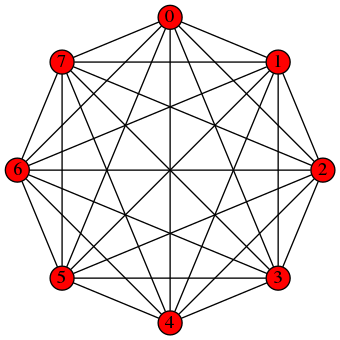
\includegraphics[scale=0.35]{figs/K8_1.png} 
%\caption{Image A}
\end{minipage}
\hfill
\begin{minipage}[c]{0.5\linewidth}
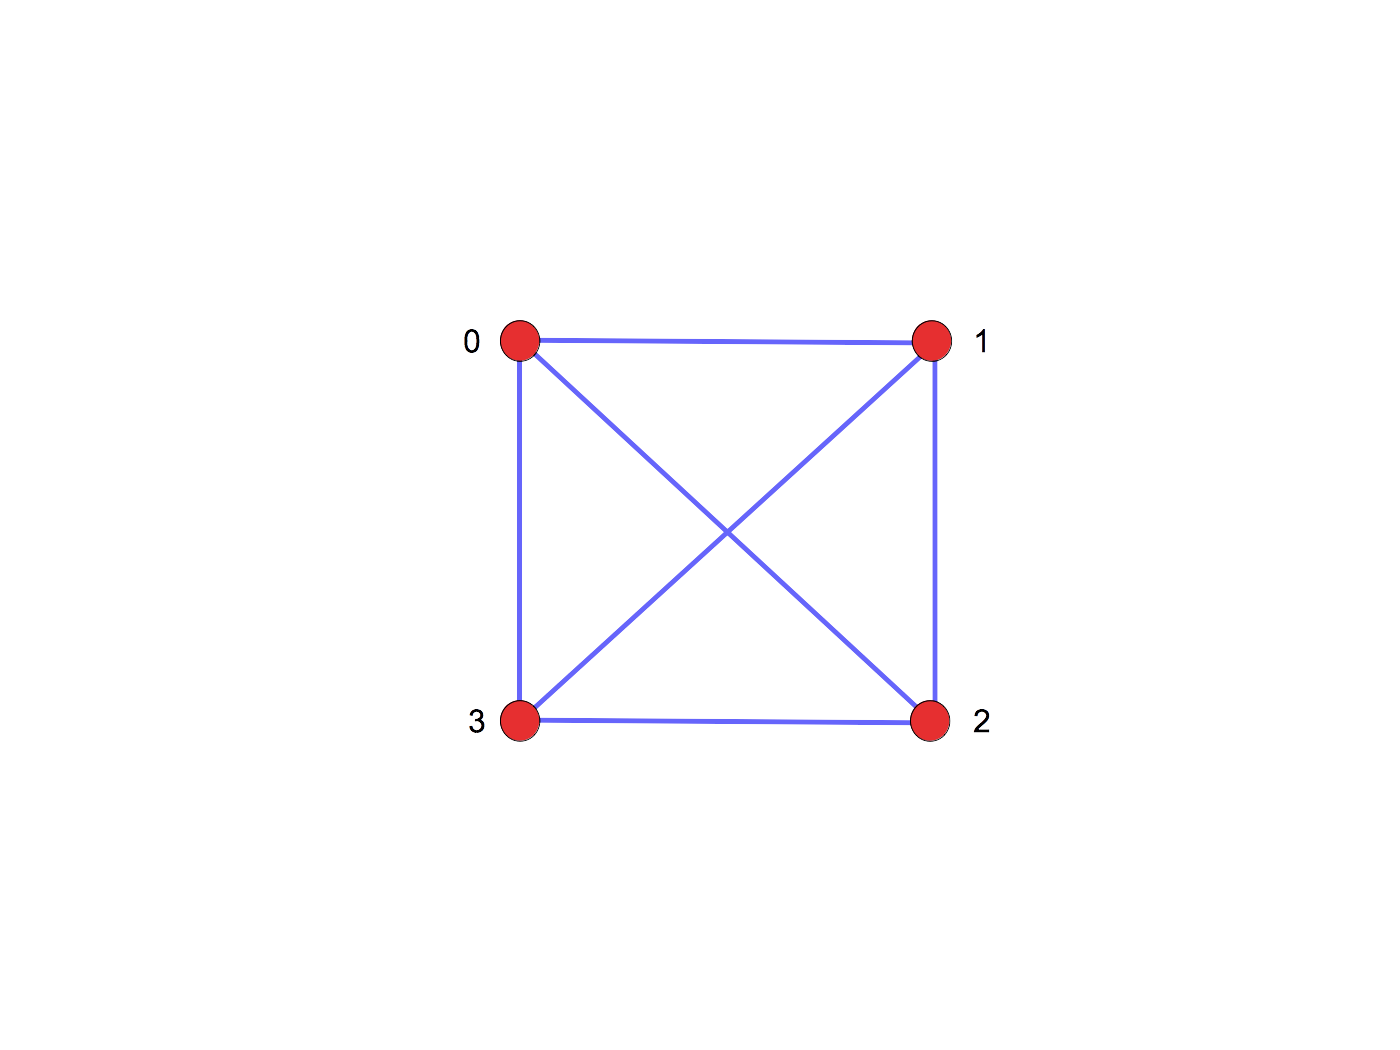
\includegraphics[scale=0.40]{figs/K4.png} 
%\caption{Image B}
\end{minipage}
\vskip-1.0cm
\caption{\footnoteskip
  The left panel shows the fully connected graph $K_8$ and the right panel 
  shows the corresponding graph $K_4$. To perform a calculation to 8-bit
  accuracy requires the connectivity of $K_8$.  We take the vertex and edge 
  sets for be $K_8$ to ${\cal V}_8 = \{0, 1, 2, \cdots, 7 \}$ and ${\cal E}_8 = 
  \{ \{ 0, 1 \}, \{ 0, 2 \},  \cdots , \{ 0 , 7\} ,  \{ 1, 2 \} ,\{ 1, 3\} , \cdots,  
  \{\, 6 , 7\}\, \}$. To perform a calculation to 4-bit accuracy requires $K_4$ 
  connectivity,  and similarly, the vertex and edge sets for $K_4$ are 
  ${\cal V}_4 = \{0, 1, 2, 3 \}$ and ${\cal E}_4 = \{    \{ 0, 1\}, \{ 0, 2\}, 
  \{ 0, 3\}, \{ 1, 2\}, \{ 1, 3\}, \{ 2, 3\}    \} $.
}
\label{fig_K8_K4}
\end{figure}
%
The left panel shows 
the completely connected graph $K_8$, with vertex and  edge sets 
%
\begin{eqnarray}
  {\cal V}_8 &=& \{0, 1, 2, \cdots, 7 \}
  \\
  {\cal E}_8 &=& 
  \{ \{ 0, 1 \}, \{ 0, 2 \},  \cdots , \{ 0 , 7\} ,  \{ 1, 2 \} , \cdots,  \{ 1, 7\} , 
  \cdots,  \{\, 6 , 7\}\, \}
  \ ,
  \nonumber \\
\end{eqnarray}
%
while the right panel shows the $K_4$ graph, 
%
\begin{eqnarray}
  {\cal V}_4 &=& \{0, 1, 2, 3 \}
  \\
  {\cal E}_4 &=& \{  \{ 0, 1\}, \{ 0, 2\}, \{ 0, 3\}, \{ 1, 2\}, \{ 1, 3\}, \{ 2, 3\}    \} 
  \ .
\end{eqnarray}
%

Rather than summing over an ordered edge set, i.e., 
%
\begin{eqnarray}
  H[Q] 
  &=&
  \sum_{r \in {\cal V}_\smR} A_r \, Q_r
  +
  \sum_{rs \in {\cal E}_\smR  }  B_{rs} \, Q_r Q_s
  \\[5pt]
  &=&
  \sum_{r=0}^{R-1} A_r\, Q_r
  +
  \sum_{r=0}^{R-1}  \sum_{s > r}^{R-1} B_{r s} \, Q_r Q_s
  \ ,
\end{eqnarray}
%
we find it convenient to sum over all values of $r$ and $s$ taking $B_{rs}$ to be symmetric. 
In this case, the double sum differs by a factor of two relative to summing over the edge 
set of the graph, 
%
\begin{eqnarray}
  H[Q] 
  &=&
  \sum_{r=0}^{R-1} A_r\, Q_r
  +
  \sum_{r=0}^{R-1}  \sum_{s = 0}^{R-1} \frac{1}{2}\, B_{r s} \, Q_r Q_s
  \ .
\end{eqnarray}
%
Furthermore, for $r = s$, there will be a linear contribution from the idempotency 
condition $Q_r^2 = Q_r$, so that
%
\begin{eqnarray}
  H[Q] 
  &=&
  \sum_{r=0}^{R-1} \left [A_r  + \frac{1}{2}\,B_{rr} \right]\, Q_r
  +
  \sum_{r=0}^{R-1}  \sum_{s \ne r , s=0}^{R-1} 
  \frac{1 }{2}\, B_{r s} \, Q_r Q_s
  \ .
\end{eqnarray}
%
We can write this as 
%
\begin{eqnarray}
  H[Q] 
  &=&
  \sum_{r=0}^{R-1}  \tilde A_r\, Q_r
  +
  \sum_{r=0}^{R-1}  \sum_{s \ne r , s=0}^{R-1} 
  \tilde B_{r s} \, Q_r Q_s
  \ .
\end{eqnarray}
%
%

%%\pagebreak

%
\section{Embedding the QUBO Problem on the Chimera Chip}
\label{sec_embedding}

\subsection{General Considerations}
The D-Wave Chimera chip consists of coupled bilayers of micro rf-SQUIDs overlaid in such a way 
that, while relatively easy to fabricate, results in a fairly limited set of physical connections between 
the qubits. However, by {\em chaining} together well chosen qubits in a positively correlated manner, 
this limitation can largely be overcome. The process of chaining requires that we (i) embed the 
logical graph onto the physical graph of the chip (for example $K_4$ onto $C_8$) and that we 
(ii) assign weights and strengths to the physical graph embedding in such as a way as to preserve 
the ground state of the logical system. These steps are called graph embedding and Hamiltonian 
embedding, respectively. 

%
\begin{figure}[h!]
\begin{minipage}[c]{0.4\linewidth}
%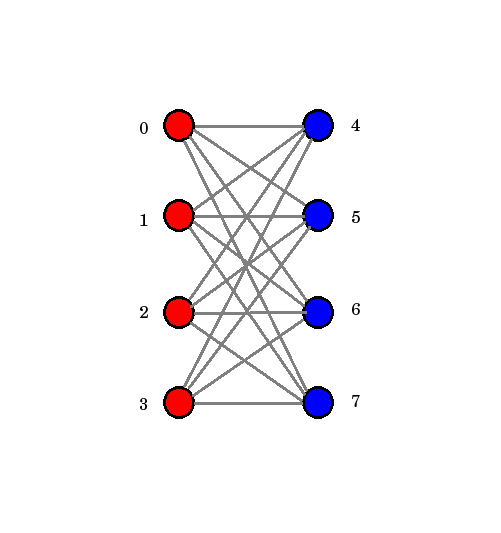
\includegraphics[scale=0.40]{figs/unit_cell0.png}
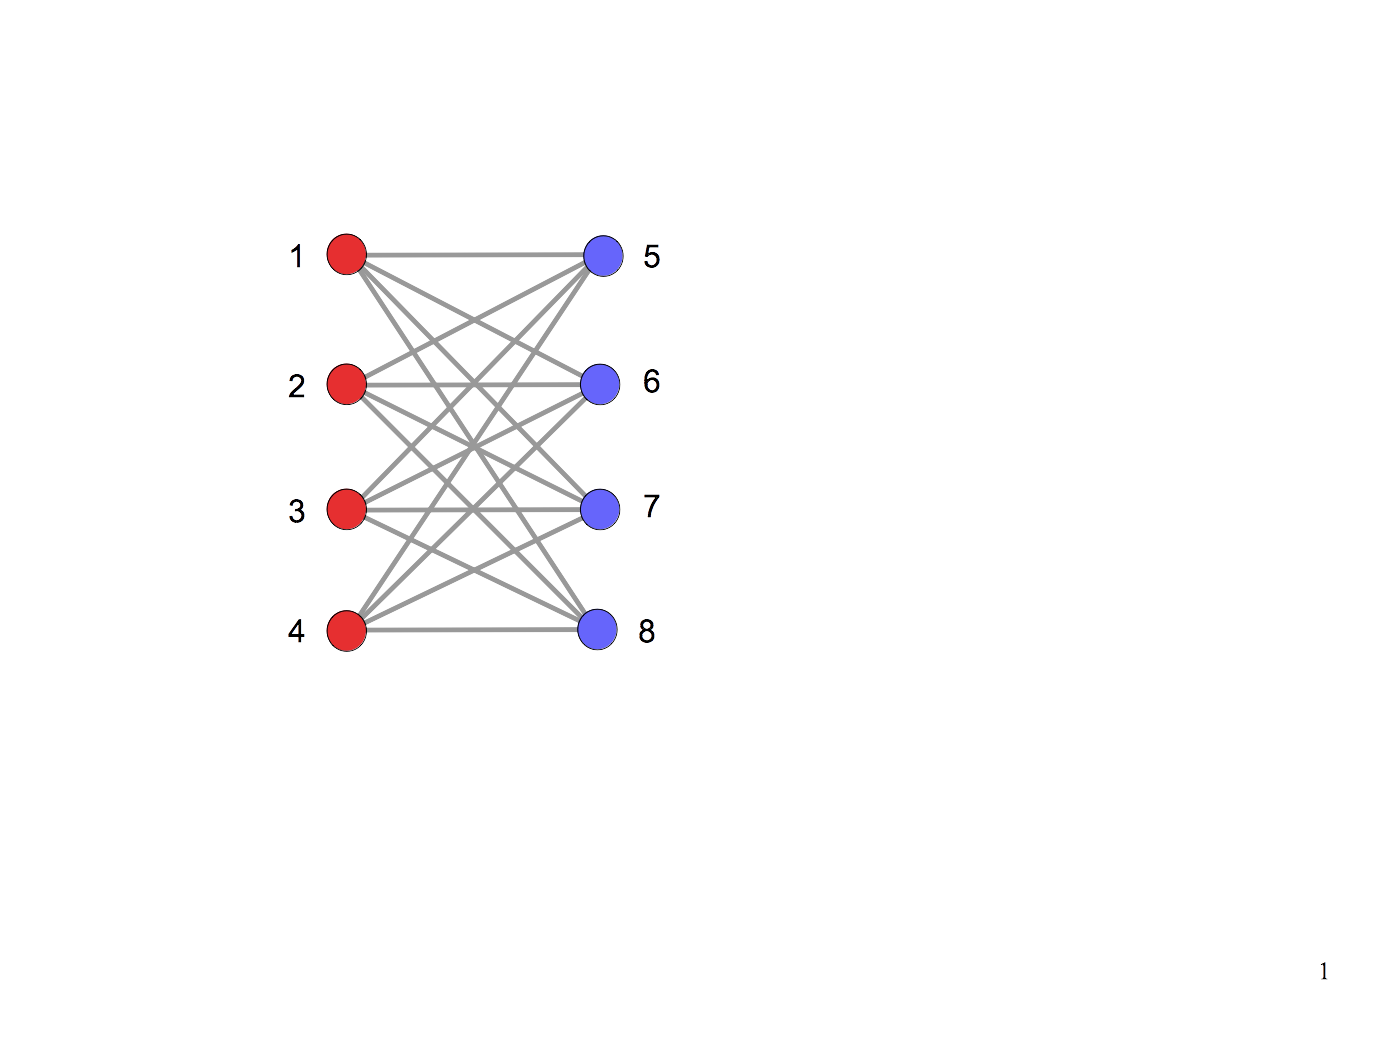
\includegraphics[scale=0.40]{figs/bipartate8_0.png}
%\caption{Image A}
\end{minipage}
\hfill
\begin{minipage}[c]{0.4\linewidth}
%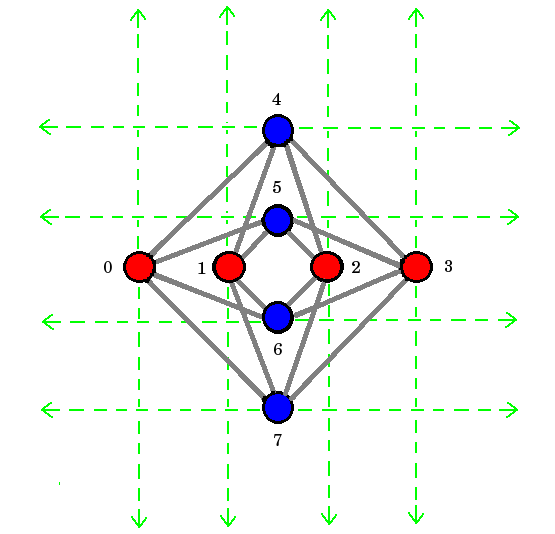
\includegraphics[scale=0.35]{figs/unit_cell1.png}
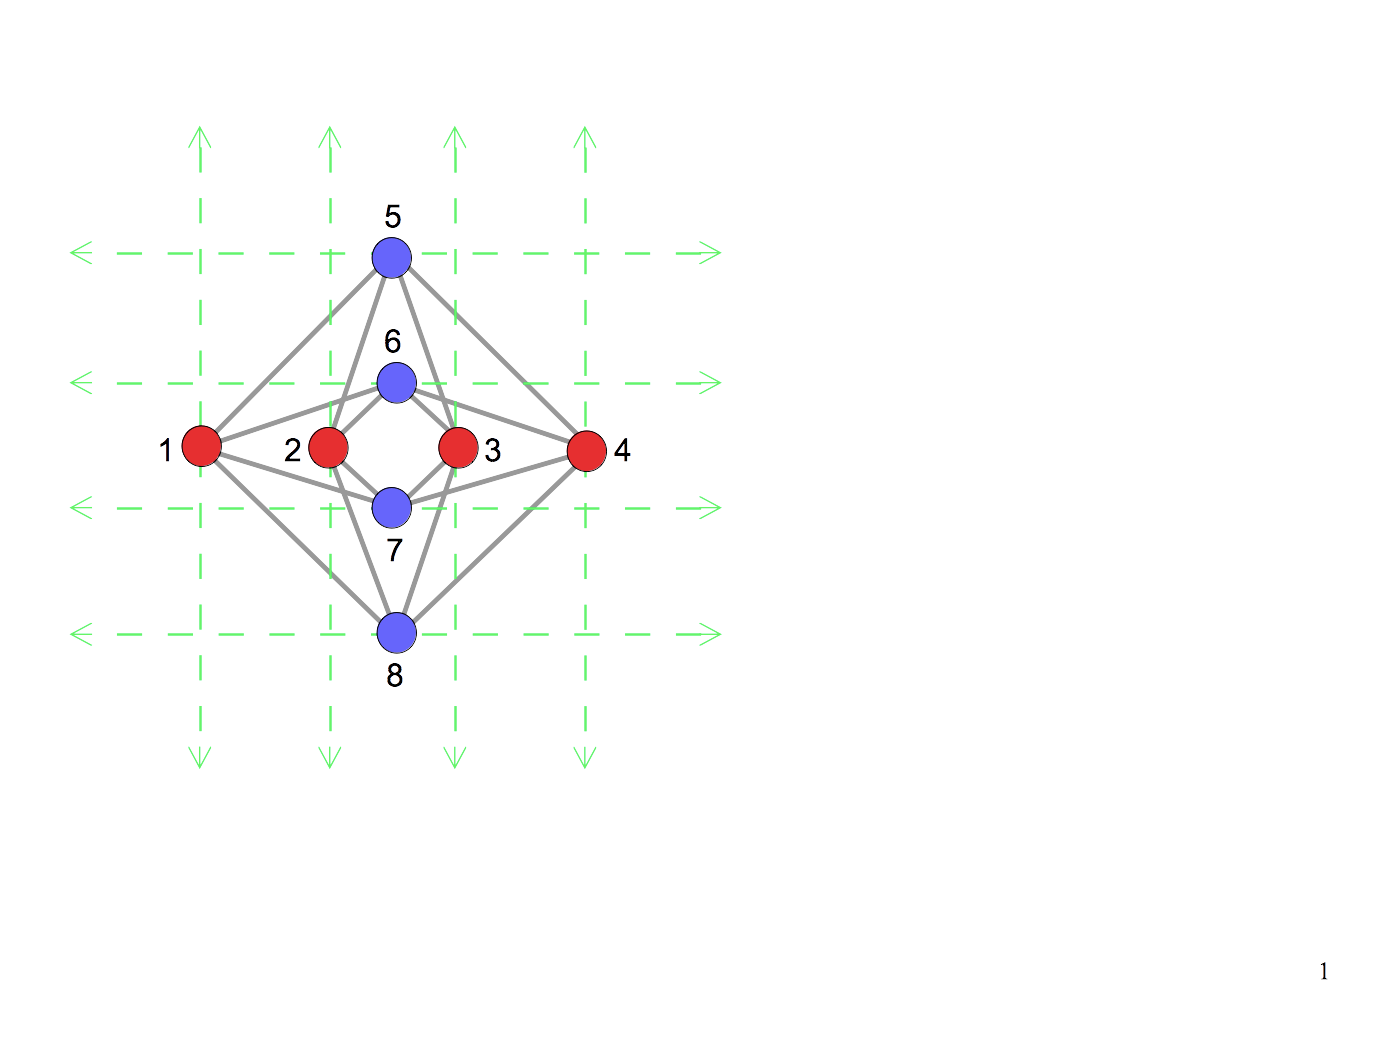
\includegraphics[scale=0.35]{figs/bipartate8_1.png}
%\caption{Image B}
\end{minipage}
\vskip-2.0cm
\caption{\footnoteskip
The left panel illustrates the bipartate graph $C_8$ in {\em column} format, 
while the right panel illustrates the corresponding graph in {\em cross} format,
often called a Chimera graph. The gray lines represent direct connections 
between qubits. The cross format is useful since it minimizes the number 
intersecting connections. The use of red and blue dots emphasize the bipartate 
nature of $C_8$, as every red dot is connected to every blue dot, while none 
of the red and blue dots are connected to one another. The vertex set of
$C_8$ is taken to be ${\cal V}_8 = \{1, 2, \cdots, 8 \}$ and edge set is 
${\cal B}_8 = \{ \{1, 5\} , \{1, 6\} , \{1, 7\} , \{1, 8\} , \{2, 5\} ,\{2, 6\} 
\cdots \{ 7, 8\} \}$. 
}
\label{fig_chimera_topology}
\end{figure}
%

%
\begin{figure}[h!]
\begin{minipage}[c]{0.4\linewidth}
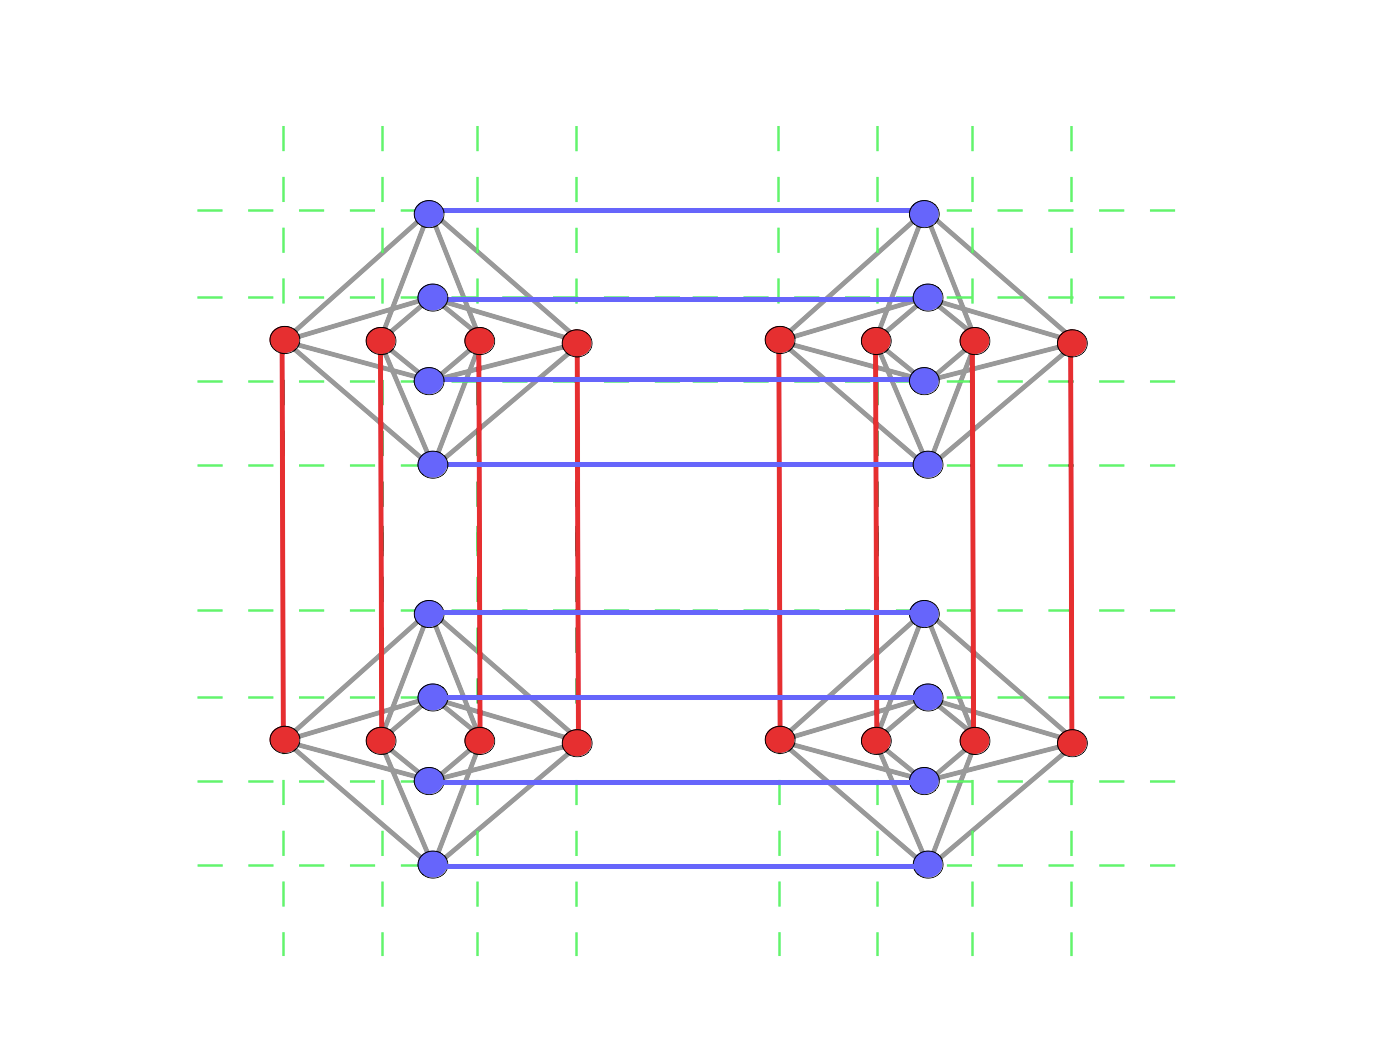
\includegraphics[scale=0.30]{figs/bipartate8_connect.png}
%\caption{Image A}
\end{minipage}
\hfill
\begin{minipage}[c]{0.4\linewidth}
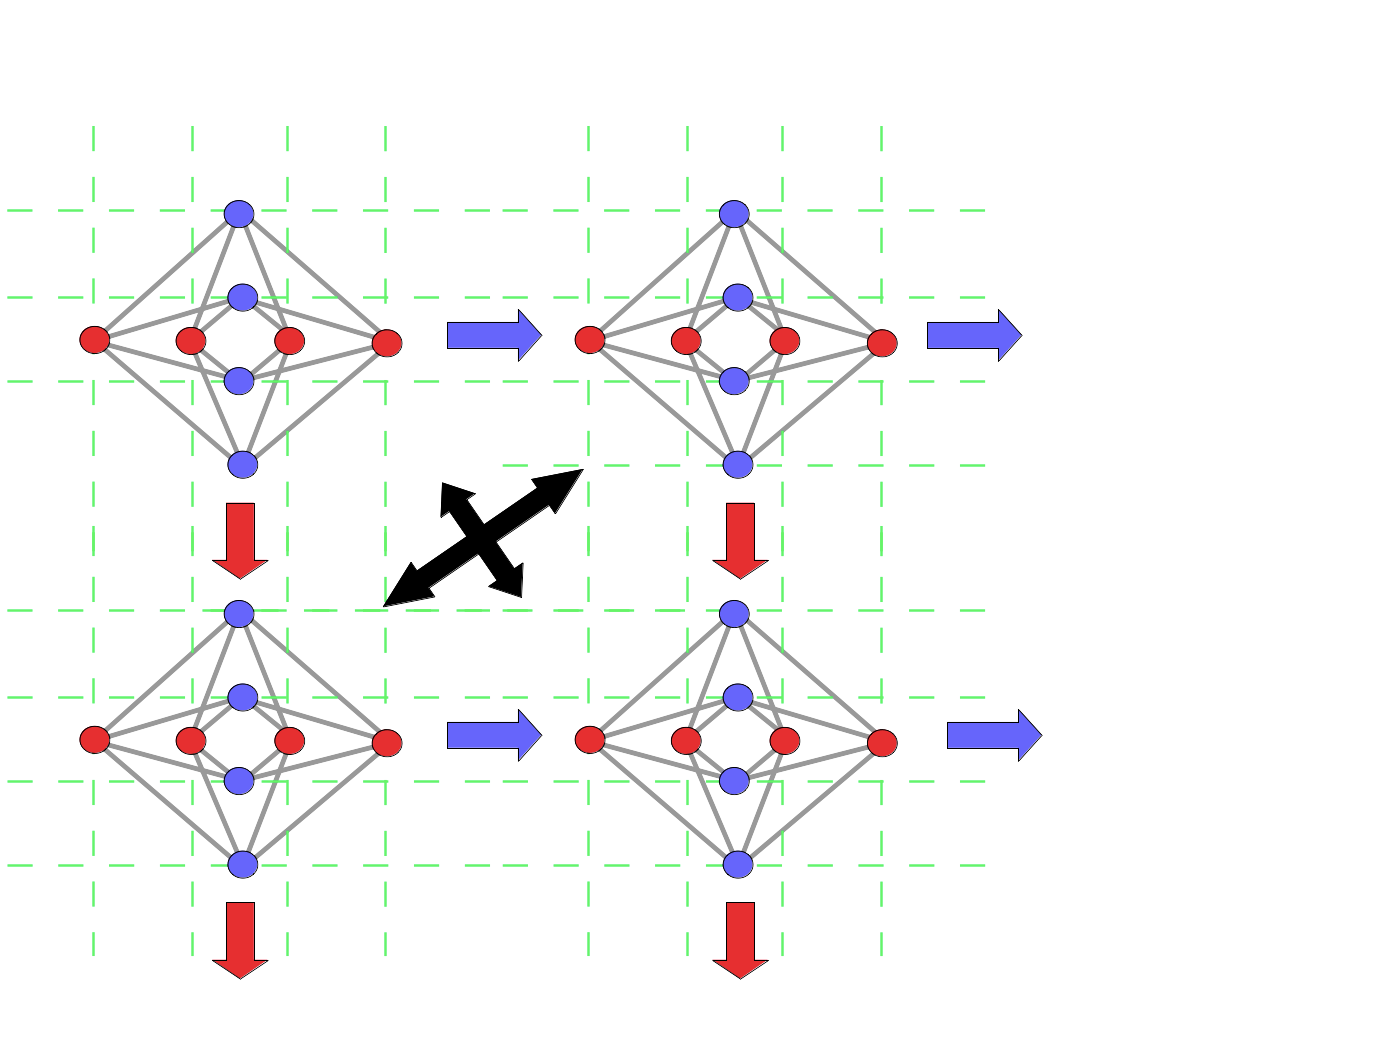
\includegraphics[scale=0.28]{figs/bipartate8_connect_diagonal.png}
%\caption{Image B}
\end{minipage}
\caption{\footnoteskip
The the left panel shows the connectivity between four $C_8$ bipartate 
Chimera zones, and the right panel illustrates how multiple $C_8$
graphs are stitched together along the vertical and horizontal
directions to provide thousands of possible qubits. A limitation of
this connectivity strategy is that red and blue zones cannot
communicate directly with one another, as indicated by the black
crossed arrows. The purpose of {\em chaining} is to allow
communication between the read and blue qubits.  
}
\label{fig_bipartate8_connect}
\end{figure}
%
Let us explore the connectivity of the D-Wave Chimera chip in more detail. The D-Wave 
architecture employs the $C_8$ bipartate Chimera graph as its most basic unit of connectivity.  
This {\em unit cell } is illustrated in Fig.~\ref{fig_chimera_topology}, and consists of 8 qubits 
connected in a $4 \times 4$ bipartate manner. The left panel of the figure uses a {\em column} 
format in laying out the qubits, and the right panel illustrates the corresponding qubits in a 
{\em cross} format, where the gray lines represent the direct connections between the qubits. 
The cross format is useful since it minimizes the number intersecting connections. The complete 
two dimensional chip is produced by replicating  $C_8$ along the vertical and horizontal 
directions, as illustrated in Fig.~\ref{fig_bipartate8_connect}, thereby providing a chip with 
thousands of qubits. The connections between qubits are limited in two ways: (i) by the 
connectivity of the basic unit cell $C_8$ and (ii) by the connectivity between the unit cells 
across the chip. The bipartate graph $C_8 = ( {\cal V}_8, {\cal B}_8 )$ is formally defined by
the vertex set ${\cal V}_8=\{1, 2, \cdots, 8 \}$, and the edge set
%
\begin{eqnarray}
  {\cal B}_8 
  &=& 
  \big\{ \{1, 5\} , \{1, 6\} , \{1, 7\} , \{1, 8\} , 
  \{2, 5\} ,\{2, 6\} , \{2, 7\}  , \{2, 8\} ,
  \nonumber
  \\
  && 
  ~~
  \{3, 5\} ,\{3, 6\} , \{3, 7\}  , \{3, 8\} ,
  \{4, 5\} ,\{4, 6\} , \{4, 7\}  , \{4, 8\} 
  \big\}. 
  \label{eq_bipartate_eight}
\end{eqnarray}
%
The set ${\cal B}_8$  represents the connections between a given red qubit and 
the corresponding blue qubits in the Figures. The red and blue dots illustrate the 
bipartate nature of $C_8$, as every red dot is connected to every blue dot, while 
none of the blue and red dots are connected to one another. 

%%\subsection{Notation Convention for Embedded and Logical Qubits}
We will denote the {\em physical} qubits on the D-Wave chip by $q_\ell$. For 
the D-Wave 2000Q there is a maximum of 2048 qubits, while the D-Wave 2X 
has 1152 qubits. For the example calculation in this text, we only use 10 to 
50 qubits. The physical Hamiltonian or objective function takes the form
%
\begin{eqnarray}
  H[q] = \sum_\ell a_\ell \, q_\ell + \sum_{\ell \ne m} 2 b_{\ell m} \, q_\ell q_m
  \ ,
\end{eqnarray}
%
where we have introduced a factor of 2 in the strength  to account for the 
symmetric summation over $r$ and $s$. We will call the qubits $Q_r$
of the previous section the {\em logical  qubits}. To write a program for the
D-Wave means finding an embedding of the logical problem onto
the physical collection of qubits $q_\ell$. If the connectivity of the Chimera 
graphs were large enough, then the logical qubits would coincide exactly with 
the physical qubits. However, since the graph $C_8$ possesses less connectivity 
than $K_4$,  we must resort to chaining on the D-Wave, even for
4-bit resolution. Figure~\ref{fig_K4_embedding_1} illustrates the $K_4$ embedding 
used by our algorithm, where, as before, the left panel illustrates the bipartate 
graph in column format, and the right panel illustrates the corresponding graph 
in cross format. 
%
\begin{figure}[h!]
\begin{minipage}[c]{0.4\linewidth}
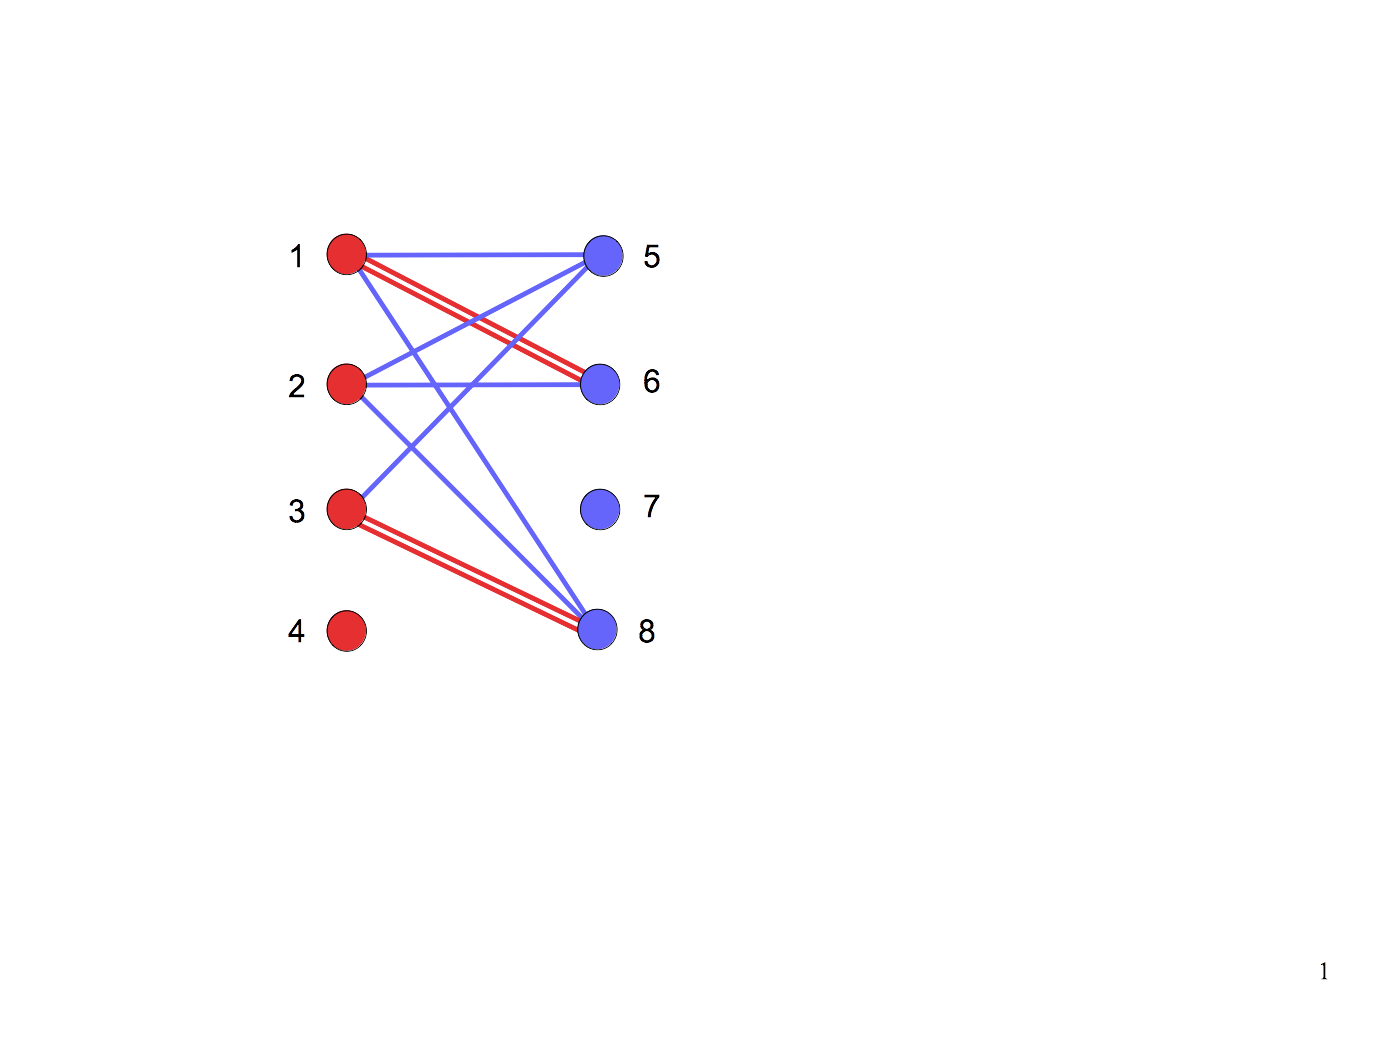
\includegraphics[scale=0.40]{figs/K4_embedding_0.png}
%\caption{Image A}
\end{minipage}
\hfill
\begin{minipage}[c]{0.4\linewidth}
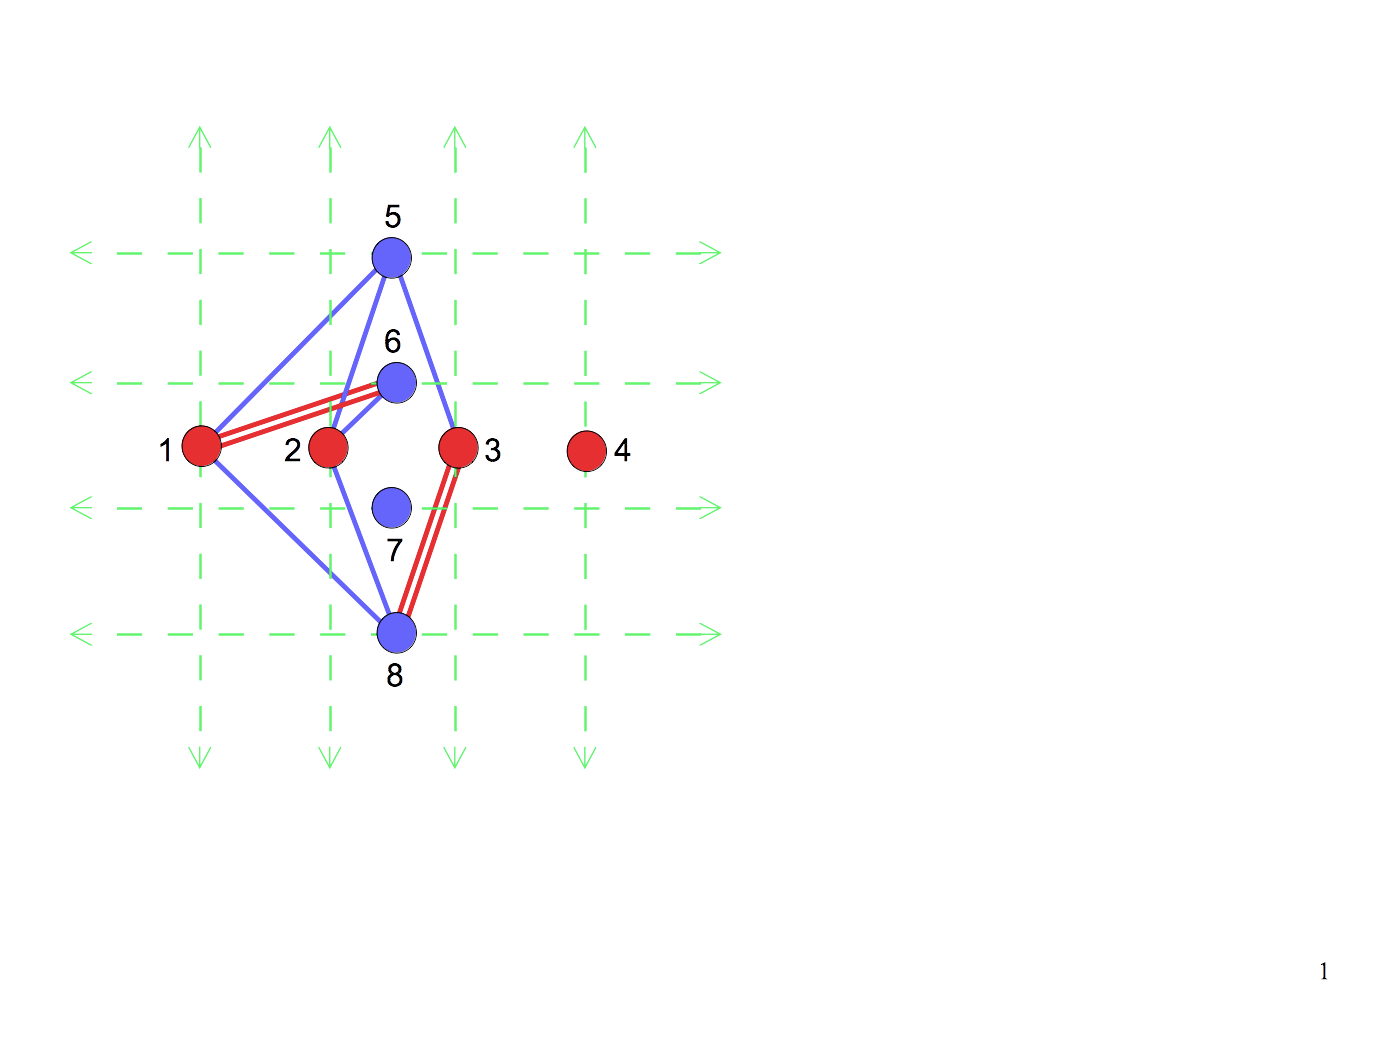
\includegraphics[scale=0.35]{figs/K4_embedding_1.png}
%\caption{Image B}
\end{minipage}
\vskip-2.0cm
\caption{\footnoteskip
The $K_4$ embedding onto $C_8$ used in our implementation 
of 4-bit of division on the D-Wave. The blue lines represent normal connections 
between qubits, while the red double-lines represent chained qubits, that is 
to say, qubits that are strictly correlated (and can thereby represent a  single 
logical qubit at a higher level of abstraction). The qubits 1-6 are chained
together, as are the qubits 3-8.
}
\label{fig_K4_embedding_1}
\end{figure}
%
\begin{figure}[h!]
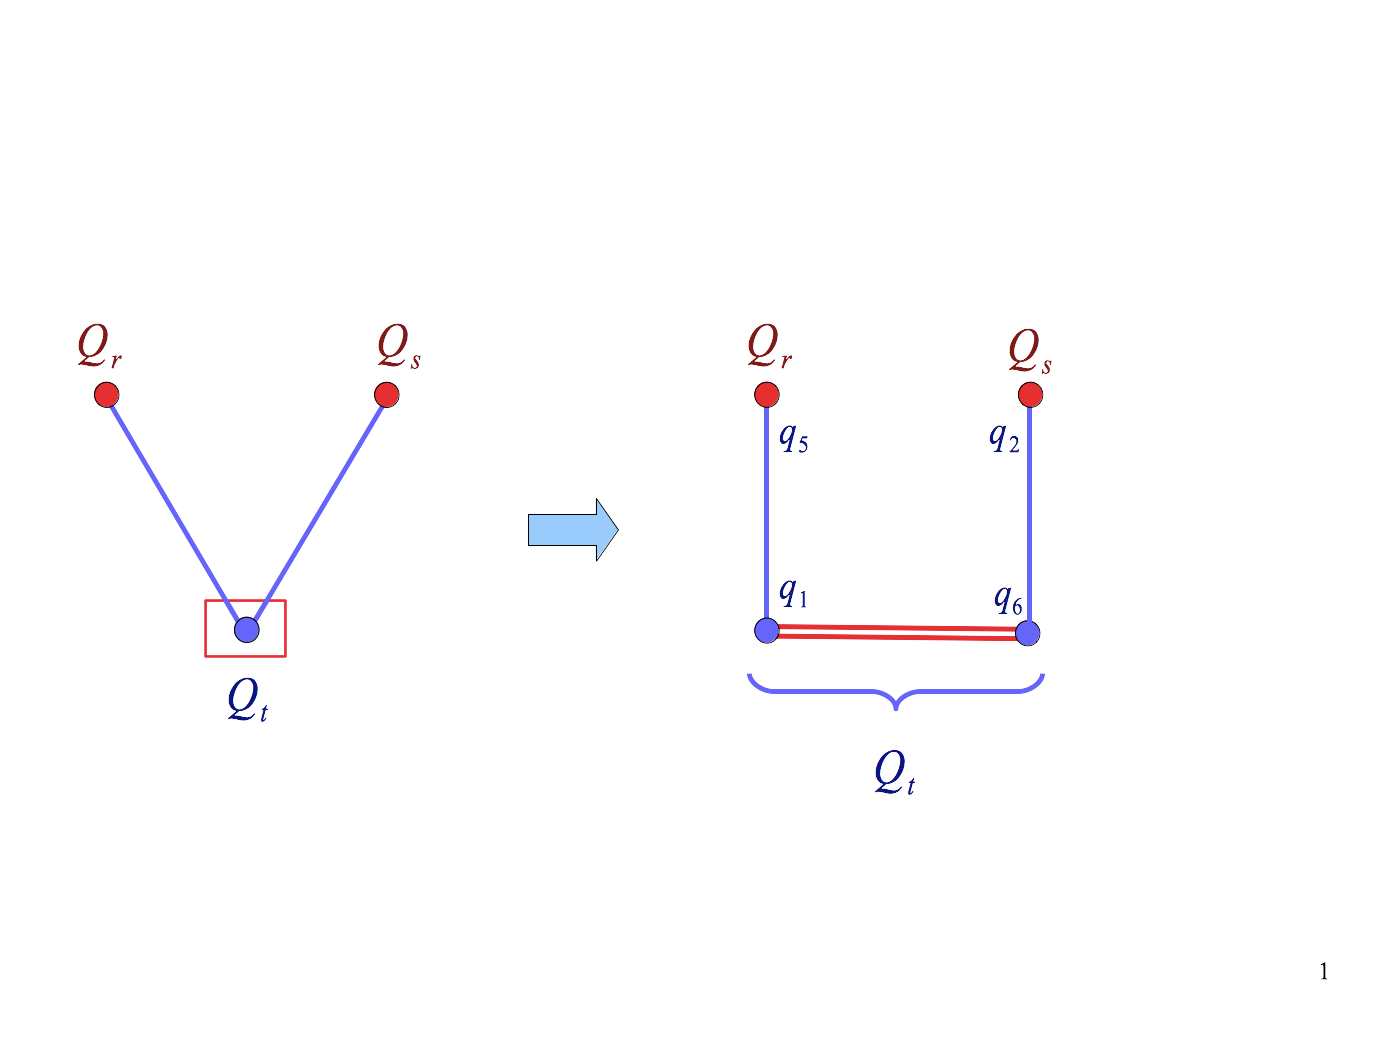
\includegraphics[scale=0.40]{figs/linear_chain_linear.png} 
\vskip-2.0cm
\caption{\footnoteskip  
The left panel shows three logical qubits $Q_r$, $Q_s$, $Q_t$ with connectivity 
between $r$-$t$ and $t$-$s$. The box surrounding qubit $t$ means that it
will be modeled by a linear chain of physical qubits, as illustrated in the right
panel. The labeling is taken from Fig.~\ref{fig_K4_embedding_1} for qubits
5-1-6-2, where $Q_r$ is mapped to $q_5$, $Q_s$ is mapped to $q_2$, and
$Q_t$ is split between $q_1$ nd $q_6$. Qubits $q_1$ and $q_6$ are chained 
together to simulate the single logical qubit $Q_t$, while qubits $Q_r$ and 
$Q_s$ map directly onto physical qubits $q_5$ and $q_2$.
}
\label{fig_linear_chain_a}
\end{figure}
%

\subsection{Chaining Strategies}
\subsubsection{The Standard Approach}
In Fig.~\ref{fig_K4_embedding_1} we have labeled the physical qubits by 
$\ell=1, 2, 3 \cdots 8$, and we wish to map the logical problem involving 
$Q_r \, Q_s \, Q_t$  onto the four physical qubits $q_5 \,q_1 \, q_6 \, q_2$. 
The embedding requires that we {\em chain}  together  the two qubits 1-6 
and 3-8, respectively. We may omit qubits $4$ and $7$ entirely. 
As illustrated in Fig.~\ref{fig_linear_chain_a}, the physical qubits $q_1$ and $q_6$ 
are {\em chained} together to simulate a single logical qubit $Q_t$, while qubits 
$q_5$ and $q_2$ are mapped directly to the logical qubits $Q_r$ and $Q_s$, 
respectively. Qubit $q_5$ is assigned the weight $a_5 = A_r$ and the coupling 
between $q_5$ and $q_1$ is assigned the value $b_{51}=B_{rt}$. Similarly for 
qubit $q_2$, the vertex is assigned weight $a_2 =  A_s$, and strength between 
$q_2$ and $q_6$ is $b_{26}=B_{st}$. We must now distribute the logical qubit 
$Q_t$ between $q_1$ and $q_6$ by assigning the values $a_1$, $a_6$ and 
$b_{16}$. We distribute the weight $A_t$ uniformly between qubits $q_1$ and 
$q_2$, giving $a_1 = A_t/2$ and $a_6 = A_t/2$. We must now choose $b_{16}$.
In this standard approach, as described in the D-Wave documentation, this
is accomplished, this is simply the negative chain penalty term, $-\alpha$.

Using superscripts to denote {\em logical qubit} indices, we may summarize 
the standard SAPI approach as,
%
%
\begin{eqnarray}  
  \label{standardweight}   
  a^t_r &=& A_t/N_t \\
  \label{standardstrength}  
  b^{r,s}_{i ,j} &=& \left\{ \begin{array}{11}  
             B_{r,s}/\nu_{r,s},  & \mbox{if $q_i \in Q_r$ and $q_j \in Q_s$} \\
             0,        & \mbox{otherwise}                 
             \end{array} \\  
  \label{standardchain}  
  b^t_{i ,i+1} &=& \left\{ \begin{array}{11} 
             -\alpha,  & \mbox{if $q_i, q_{i+1} \in Q_t$}\\
             0,        & \mbox{otherwise}             
             \end{array}
 %\\[8pt]
\,
\end{eqnarray}
%
where,
%
\begin{eqnarray}
  N_t &:=& \mbox{The number of physical qubits in the logical qubit $Q_t$} \\
  \nu_{r,s} &:=& \mbox{The number of physical qubits coupling logical qubits $Q_r$ and $Q_s$}.
\end{eqnarray}
%

%%where $N_t$ is the number of physcial qubits in logical qubit $Q_t$, and $\nu_{r,s}$
%%is the number of physical qubits that are actually coupled between the logical qubits $Q_r$ and $Q_s$.
Usually, the default SAPI embedding will give all $\nu_{r,s}=1$, that is, only one
pair of physical qubits is actually coupled to embody the logical qubit coupling, $B_{r,s}$.
However, occasionally the SAPI embedding function will couple together two qubits
across a pair of logical qubits, in which case it will set the value of each 
coupling term to the above form with $\nu=2$. We will assume from now on that all
logical qubits are coupled by only one pair of physical qubits, but this is not
essential to the following discussion.

Note that this standard chaining scheme will generally give a total energy that
is different than that for the corresponding logical Hamiltonian. To see this, first assume that none
of the chains are broken, so that $q_i = Q_r$ for all $q_i$ contain within the logical qubit $Q_r$.
Then, the ground state for this chaining scheme will differ from the ground state 
in terms of logical qubits by an additive perturbation.  For a problem with $N$ logical
qubits, each consisting of $N_t$ physical qubits that are chained together within logical qubit $Q_t$, 
we can see by inspection that the perturbed ground state energy can be written as,
%
\begin{eqnarray}
  E_0[q^0_i] = E_0[Q^0_t] + \Delta E
\end{eqnarray}\\
%
where,
%
\begin{eqnarray}
  \Delta E &:=& \sum_{chains} -\alpha \times (\mbox{the number of links}) \\
           &=& -\alpha \times \sum_{t=1}^N (N_t-1)
  \label{perturbation}
\end{eqnarray}\\
%
where,
Here, the subscript $0$ refers to values in the ground state.  The expression derives 
from the fact that there is a contribution of $-\alpha$ from each ``link'' in the 
chain, and there are $N_t-1$ links.  Note that this relation would actually
hold for every state in the spectrum of the Hamiltonian in logical qubits when there are no
unbroken chains.

Observe two things: (1) The ground state energy with all the physical qubits included will 
be lower than that for that for the logical qubits when there are no unbroken chains, and;
(2) The magnitude of the perturbation, $\Delta E$, depends on the values of the particular
$N_t$ values, which depends on the particular graph embedding employed. So, one problem is that
the perturbation is a function of the graph embedding. The same problem with a different embedding
onto the Chimera graph could give a different energy perturbation.

But note, also, that, frequently, there may be very small energy differences resulting from reversals of only
a few of the physical qubits in ground state. This typically occrus when there are many near cancellations
in energy, so that simultaneous reversal of a pair or group of qubit values within possibly different chains
may result in a net lower energy if the corresponding chain perturbation is lower than
the other terms in the Hamiltonian involving those qubits. This will generally happen when the 
chaining penalty is too small to compensate for these energy differences. This possiblity should be
obvious by just considering that the chaining penalty must be set large enough to bias the physical
qubits to positive correlations or they will not chain together. However, the chaining penalty 
cannot be made arbitrarily large, either.  If there are many states of the embedded system with 
energies close to the ground state, the chaining penalty may need to be set to tens or hundreds 
of times the values some of the $A_t$ and $B_{r,s}$ parameters to chain physical qubits into
logical qubits. But then, when the Hamiltonian is normalized to values within the dynamic range 
of the machine,the energies from of the some logical qubits couplings may become negligible, 
i.e., those couplings will no longer contribute significantly to the total energy. In such cases,
the solution may not represent the solution of the intended QUBO problem at all, although there
may be no broken chains. 

For a QUBO problem to be effectively solveable on the D-Wave quantum annealer, there must be feasable range of 
chaining penalties; large enough to chain the physical qubits together into logical qubits, but not drastically 
larger than the values of the strengths and weights for the logical qubits. And, for some QUBO problem Hamiltonians, 
typically those with very high spectral densities near the ground state, this is simply not possible. Some QUBO problems 
may either require longer annealing times, or more reads, or they may simply not be practically solvable on the annealer.
But it is difficult to know when a hard QUBO problem may yet be solved by longer annealing times or more cycles
if the chaining perturbation error has not been accounted for, because one generally cannnot objectively determine, a priori,
whether the reason it's not converging is primarily due to computability limitations, or the physical limitations of the device, 
such as thermal noise, or simply from the numerical errors resulting from the chaining perturbation. However, the latter 
is simply an unneccessary numerical error which is caused by trying to set the parameters without knowing anything 
about the chain sizes due to the particular graph embedding. Yet, this information is readily available after one has done 
the neccessary step of embedding the graph. Therefore, this chaining information should to be used to correct the 
chaining perturbation if one wants to have the best chance of solving any potentially difficult QUBO problem.

We address how to use the chain sizes to set the parameters in order to keep the spectrum invariant 
in the following section.


\subsubsection{The Spectrally Invariant Approach}
Clearly, to keep the spectrum invariant, we must eliminate the perturbation from the
chaining penalty.
To do that, we simply shift the values of the weights, $a_i$, using information that we 
already must have from embedding the graph onto the Chimera chip. We only need to know
the length of each chain (i.e., the size of each logical qubit), which is known from 
the graph embedding step. Then, it is straight-forward to add a counter-term to the weights 
for the physical Hamiltonian to subtract the perturbation from the chaining penalty.
The sum over link in a the chain for logical qubit $Q_t$, gives a perturbation of,
%
\begin{eqnarray}
  \Delta E_{Q_t} = -\alpha \times (N_t-1). 
  \label{qperturbation}  
\end{eqnarray}
%
As in equation~\ref{standardweight}, for each physical qubit, $q_i$ within logical qubit $Q_t$ 
we may still choose the weights to have a contribution determined by the
logical qubit weights, of the form,
%
\begin{eqnarray}
  a_i \propto \frac{A_t}{N_t},
\end{eqnarray}
%
up to a constant term chosen to cancel the chain coupling perturbation.  Clearly, the
simplest counter-term that will accomplish this is just
%
\begin{eqnarray}
  ct_i^t = \alpha \times \frac{(N_t-1)}{N_t}.
\end{eqnarray}
%
Therefore, in our spectrum preserving weighting scheme, we simply add this counter-term to the weights 
in equations~\ref{standardweight}, giving,
%
\begin{eqnarray}
  a^t_r = \frac{A_t}{N_t} + \alpha \times \frac{(N_t-1)}{N_t}.
  \label{newweight}
\end{eqnarray}
%\pagebreak

\subsubsection{Example}
We now illustrate the affect of applying the counter-term vs not applying the counter-term when embedding
a Hamiltonian. The Hamiltonian in this is example is for solving a $2$-dimensional linear equation defined by
an ill-conditioned 2x2 matrix. In such cases, the energy spectrum will have a large number of states packed
close in energy to the ground state. The energy spectrum is plotted in Fig.~\ref{fig_energy}, below.

%
\begin{figure}[h!]
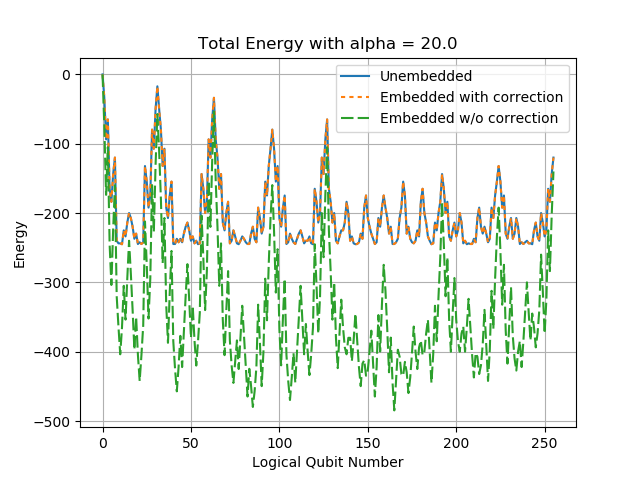
\includegraphics[scale=0.8]{figs/energy.png} 
\caption{\footnoteskip  
%
  The energy surface for a certain QUBO Hamiltonian. This is plotted for three cases:  (1) The unembedded original Hamiltonian,
  in terms of ``logical'' qubits (blue); (2) the embedded Hamiltonian with the corrected weightings, from equation~\ref{newweight} (red),
  and; (3) the embedded Hamiltonian without the corrected weightings (green).
%
}
\label{fig_energy}
\end{figure} 
%
Clearly, the correctly for inhomogeneous chain sizes matters a great deal. Note that, with the correction given by equation~\ref{newweight},
the energy spectrum (summed over the chained qubits) is exactly equilvalent to the energy spectrum for the unchained (logical) Hamiltonian.
However, without the correction added to the weights, there is a very significant difference. In fact, it changes the shape of the energy spectrum
to such a degree that the lowest energy state is significantly different from the ground state energy of the unchained Hamiltonian, so that the
uncorrected embeddiing could not be expected to yield the correct ground state for the original Hamiltonian with the embedded Hamiltonian on the
D-Wave quantum annealer.


%% %
%% \pagebreak
%% \begin{acknowledgments}
%% We received funding for this work from the {\em ASC Beyond Moore’s Law Project} 
%% at LANL.  
%% \end{acknowledgments}
%% %\pagebreak

% %\vfill
% \pagebreak
% \clearpage
% % Bibliography
% \begin{thebibliography}{99}
% \bibskip

% \bibitem{hhl}
%   A. Harrow, A. Hassidim, and S. Lloyd, 
%   Phys. Rev. Lett. {\bf 103}, 150502 (2009). 

% \bibitem{ref2013a}
%   Stefanie Barz, Ivan Kassal, Martin Ringbauer, Yannick Ole Lipp, Borivoje Dakic ́, 
%   \hbox{Ala ́n} Aspuru-Guzik, Philip Walther, 
%   {\em  Solving systems of linear equations on a quantum computer},
%   arXiv:1302.1210v1 (2013).  

%   \bibitem{ref2013b}
%   Stefanie Barz, Ivan Kassal, Martin Ringbauer, Yannick Ole Lipp, Borivoje Dakic ́,
%    Ala ́n Aspuru-Guzik, Philip Walther, 
%   {\em  Solving systems of linear equations on a quantum computer},
%   arXiv:1302.1946v1 (2013).

% \bibitem{ref2013c}
%   X.-D. Cai, C. Weedbrook, Z.-E. Su, M.-C. Chen, Mile Gu, M.-J. Zhu, Li Li, 
%   Nai-Le Liu, Chao-Yang Lu, Jian-Wei Pan, 
%   {\em  Experimental quantum computing to solve systems of linear equations},
%   arXiv:1302.4310v2 (2013).  

% \bibitem{fggs}
%   Edward Farhi, Jeffrey Goldstone, Sam Gutmann and Michael Sipser,
%   {\em Quantum Computation by Adiabatic Evolution},
%   arXive:000110 (2000). 

% \bibitem{Ising1925}
%   E. Ising,  {\em Z. Phys.} {\bf 31} (1925) 253.
 
% %\bibitem{annealing_gated}
% %  Yigit Subasi and Rolando D. Somma,
% %  {\em Quantum algorithms for linear systems of equations inspired by adiabatic quantum computing},
% %  arXiv:1805.10549. 

% \bibitem{gray_code}
%   Press, William H.; Teukolsky, Saul A.; Vetterling, William T.; Flannery, Brian P. 
%   {\em "Section 22.3. Gray Codes". Numerical Recipes: The Art of Scientific Computing (3rd ed.)},
%   New York, USA: Cambridge University Press. ISBN 978-0-521-88068-8 (2007).

% \bibitem{messiah}
%   Messiah, Albert
%   {\em ``Chapter XVII.'' Quantum Mechanics.}
%   Dover Publications. ISBN 0-486-40924-4. (1999)

% \end{thebibliography}
% %

\end{document}
